\documentclass[11pt]{article}
\usepackage[margin=1in]{geometry}
\usepackage[utf8]{inputenc}
\usepackage[T1]{fontenc}
\usepackage{lmodern}
\usepackage{amsmath,amssymb,amsthm}
\usepackage{tikz}
\usepackage[title]{appendix}
\usepackage[colorlinks=true,linkcolor=blue,citecolor=blue,urlcolor=blue,pdfauthor={P. Graham},pdftitle={The Heawood family is not the complete list of excluded minors for Colin de Verdière invariant at most 5}]{hyperref}
\newtheorem{theorem}{Theorem}
\newtheorem{corollary}[theorem]{Corollary}
\newtheorem{lemma}[theorem]{Lemma}
\theoremstyle{remark}
\newtheorem{remark}[theorem]{Remark}
\setlength{\emergencystretch}{3em}
\title{The Heawood family is not the complete list of excluded minors for Colin de Verdière invariant at most 5}
\author{P. Graham\\ \small\url{https://orcid.org/0009-0007-8493-1505}}
\date{November 11, 2026}
\begin{document}
\maketitle
\begin{abstract}
We show that two intrinsically knotted graphs $G_1$ and $G_2$ with 23
edges, on 11 and 12 vertices, have Colin de Verdière invariant $\mu=6$ and
no minor in the Heawood family, the 78 graphs obtained from $K_7$ and
$K_{3,3,1,1}$ by $\Delta Y$- and $Y\Delta$-transformations. So the Heawood
family is not the complete list of excluded minors for $\mu\le5$, as van
der Holst proposed; Mattman and Pavelescu stated this proposal as a
conjecture and derived from it that $G_1$ and $G_2$ have $\mu=5$. More
precisely, either the common minor $H$ of $G_1$ and $G_2$, a 4-regular
graph with 11 vertices and 22 edges, is an excluded minor for $\mu\le5$, or
$G_1$ and $G_2$ both are. It follows that the following two conjectures of
van der Holst cannot both hold: (a) a graph is 4-flat if and only if
$\mu\le5$; (b) the Heawood family is the complete list of excluded minors
for 4-flat graphs. The lower bound $\mu\ge6$ is proved by explicit matrices
certified in interval and exact rational arithmetic, and the minor
exclusion by exhaustive enumeration.

This work has not yet been reviewed by experts.
The proofs, the computer checks and the text were produced by AI models
(from OpenAI and Anthropic), working under the author's direction.
\end{abstract}
\medskip
\noindent\textit{Keywords:} Colin de Verdière invariant, excluded minors,
Heawood family, 4-flat graphs, intrinsically knotted graphs.

\noindent\textit{MSC 2020:} 05C83, 05C50, 57M15, 05C10.

\section{Introduction}

\subsection{Main result}
All graphs are finite and simple, with vertex set $\{0,\dots,n-1\}$. Let
$G=(V,E)$ be a graph on $n$ vertices. Following van der Holst, Lovász and
Schrijver \cite[1.1]{HLS}, the \emph{Colin de Verdière invariant}
$\mu(G)$ is the largest corank of a real symmetric $n\times n$ matrix $M$
such that
\begin{itemize}
\item[(i)] for $i\ne j$, $M_{ij}<0$ if $ij\in E$ and $M_{ij}=0$ if
  $ij\notin E$, with no condition on the diagonal;
\item[(ii)] $M$ has exactly one negative eigenvalue, of multiplicity one;
\item[(iii)] (the Strong Arnold Property) no nonzero real symmetric matrix
  $X$ with $X_{ij}=0$ whenever $i=j$ or $ij\in E$ satisfies $MX=0$.
\end{itemize}
A \emph{minor} of a graph is a graph obtained from it by deleting vertices
and edges and contracting edges, merging parallel edges and removing loops.
Since $\mu$ does not increase under taking minors \cite{CdV}, the graphs
with $\mu\le k$ form a minor-closed class. An \emph{excluded minor} for a
minor-closed class is a graph outside the class all of whose proper minors
lie in it; a graph is in the class if and only if it has no excluded minor
as a minor. A graph is \emph{$t$-apex} if deleting at most $t$ vertices
leaves a planar graph.

A $\Delta Y$-transformation replaces the three edges of a triangle by a
new vertex adjacent to its three corners; a $Y\Delta$-transformation is the
reverse, applied to a vertex of degree three. The \emph{Heawood family}
consists of the 78 graphs obtained from $K_7$ and $K_{3,3,1,1}$ by
repeated $\Delta Y$- and $Y\Delta$-transformations \cite[\S1.1]{GW}: the
20 graphs of the $K_7$ family, with 21 edges, and the 58 of the
$K_{3,3,1,1}$ family, with 22 edges.

Let $G_1$ and $G_2$ be the graphs with these edge sets:
\begin{align*}
E(G_1)=\{&04,05,06,07,15,16,17,18,1\,10,26,27,28,29,37,38,39,3\,10,\\
&48,49,4\,10,59,5\,10,6\,10\},\\
E(G_2)=\{&05,06,08,09,15,18,19,1\,10,26,27,28,37,39,3\,10,3\,11,\\
&48,49,4\,10,4\,11,57,5\,11,6\,10,6\,11\}.
\end{align*}
$G_1$ has 11 vertices and 23 edges, nine of degree $4$ and two of degree $5$;
$G_2$ has 12 vertices and 23 edges and arises from $G_1$ by a
$\Delta Y$-transformation on the triangle $\{1,5,10\}$
(Figure~\ref{fig:graphs}). They are entries 90 and 332 (numbered from 0)
of the list of 3028 obstructions to knotless embedding in Appendix~A of
Mattman and Pavelescu \cite{MP}, and the graphs $G_2$ and $G_3$ of Kim
and Mattman \cite[\S3]{KM}. Let $H$ be the graph $G_1$ with the edge
$\{1,10\}$ deleted; it is 4-regular with 11 vertices and 22 edges.
Mattman and Pierce found $H$ by a computer search, as one of two 4-regular
graphs with 11 vertices and 22 edges that are not 2-apex while all their
proper minors are \cite[\S2]{MPi} (their second edge list, with labels
shifted by one). Kim and Mattman call it $H_2$ and show that, up to isomorphism, $H$ is the
only minor of $G_1$ or $G_2$ obtained by one edge deletion or contraction
that is not 2-apex \cite[\S\S3.1, 3.3]{KM}.

\begin{figure}[ht]
\centering
% BEGIN Figure 1, generated by checks/figure.py from data/graphs.g6
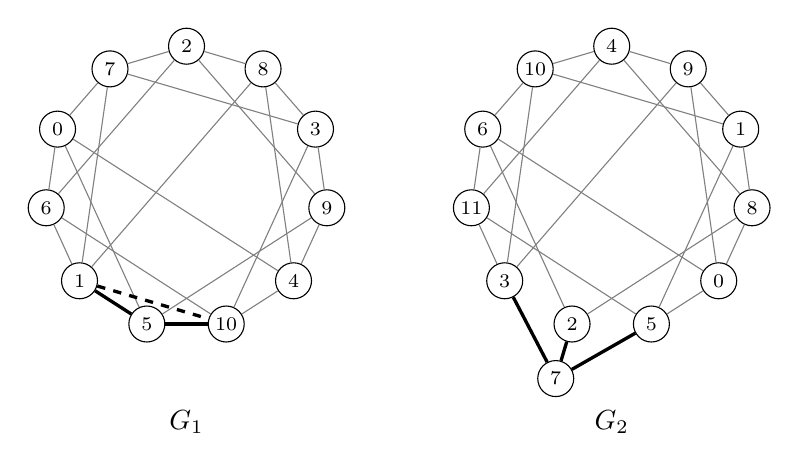
\begin{tikzpicture}[scale=0.9,v/.style={circle,draw,fill=white,inner sep=1pt,minimum size=13pt,font=\scriptsize}]
\node[v] (a0) at (-1.82,0.83) {0};
\node[v] (a1) at (-1.51,-1.31) {1};
\node[v] (a2) at (0.00,2.00) {2};
\node[v] (a3) at (1.82,0.83) {3};
\node[v] (a4) at (1.51,-1.31) {4};
\node[v] (a5) at (-0.56,-1.92) {5};
\node[v] (a6) at (-1.98,-0.28) {6};
\node[v] (a7) at (-1.08,1.68) {7};
\node[v] (a8) at (1.08,1.68) {8};
\node[v] (a9) at (1.98,-0.28) {9};
\node[v] (a10) at (0.56,-1.92) {10};
\draw[gray] (a0) -- (a4);
\draw[gray] (a0) -- (a5);
\draw[gray] (a0) -- (a6);
\draw[gray] (a0) -- (a7);
\draw[very thick] (a1) -- (a5);
\draw[gray] (a1) -- (a6);
\draw[gray] (a1) -- (a7);
\draw[gray] (a1) -- (a8);
\draw[dashed,very thick] (a1) -- (a10);
\draw[gray] (a2) -- (a6);
\draw[gray] (a2) -- (a7);
\draw[gray] (a2) -- (a8);
\draw[gray] (a2) -- (a9);
\draw[gray] (a3) -- (a7);
\draw[gray] (a3) -- (a8);
\draw[gray] (a3) -- (a9);
\draw[gray] (a3) -- (a10);
\draw[gray] (a4) -- (a8);
\draw[gray] (a4) -- (a9);
\draw[gray] (a4) -- (a10);
\draw[gray] (a5) -- (a9);
\draw[very thick] (a5) -- (a10);
\draw[gray] (a6) -- (a10);
\node[v] (b0) at (7.51,-1.31) {0};
\node[v] (b1) at (7.82,0.83) {1};
\node[v] (b2) at (5.44,-1.92) {2};
\node[v] (b3) at (4.49,-1.31) {3};
\node[v] (b4) at (6.00,2.00) {4};
\node[v] (b5) at (6.56,-1.92) {5};
\node[v] (b6) at (4.18,0.83) {6};
\node[v] (b7) at (5.21,-2.69) {7};
\node[v] (b8) at (7.98,-0.28) {8};
\node[v] (b9) at (7.08,1.68) {9};
\node[v] (b10) at (4.92,1.68) {10};
\node[v] (b11) at (4.02,-0.28) {11};
\draw[gray] (b0) -- (b5);
\draw[gray] (b0) -- (b6);
\draw[gray] (b0) -- (b8);
\draw[gray] (b0) -- (b9);
\draw[gray] (b1) -- (b5);
\draw[gray] (b1) -- (b8);
\draw[gray] (b1) -- (b9);
\draw[gray] (b1) -- (b10);
\draw[gray] (b2) -- (b6);
\draw[very thick] (b2) -- (b7);
\draw[gray] (b2) -- (b8);
\draw[very thick] (b3) -- (b7);
\draw[gray] (b3) -- (b9);
\draw[gray] (b3) -- (b10);
\draw[gray] (b3) -- (b11);
\draw[gray] (b4) -- (b8);
\draw[gray] (b4) -- (b9);
\draw[gray] (b4) -- (b10);
\draw[gray] (b4) -- (b11);
\draw[very thick] (b5) -- (b7);
\draw[gray] (b5) -- (b11);
\draw[gray] (b6) -- (b10);
\draw[gray] (b6) -- (b11);
\node at (0,-3.3) {$G_1$};
\node at (6,-3.3) {$G_2$};
\end{tikzpicture}
% END Figure 1
\caption{Left, $G_1$; deleting the dashed edge $\{1,10\}$ gives $H$.
Right, $G_2$, obtained from $G_1$ by a $\Delta Y$-transformation on the
thick triangle $\{1,5,10\}$; the new vertex is $7$ and the thick edges are
its three edges. Vertices of $G_2$ carry their labels in $G_2$. Drawn by
\texttt{checks/figure.py} from \texttt{data/graphs.g6}, which also checks
the drawing.}\label{fig:graphs}
\end{figure}

\begin{theorem}\label{thm:main}
$\mu(G_1)=\mu(G_2)=6$, and neither $G_1$ nor $G_2$ has a minor in the
Heawood family.
\end{theorem}

\begin{corollary}\label{cor:obstruction}
The Heawood family is not the complete list of excluded minors for the
class of graphs with $\mu\le5$. More precisely, if $\mu(H)=6$ then $H$
is an excluded minor for $\mu\le 5$, and otherwise $G_1$ and $G_2$ both
are; in either case none of them is in the Heawood family.
\end{corollary}

The lower bound $\mu\ge6$ rests on two certificates, one explicit matrix
for each graph, checked in exact rational and interval arithmetic, and
the minor exclusion on an exhaustive enumeration
(Section~\ref{sec:verification}). The upper bound $\mu\le6$ and the
identification of the excluded minor are short arguments from known
facts.

\subsection{Background}
Colin de Verdière proved that $\mu$ is minor-monotone and that $\mu(G)\le3$
exactly when $G$ is planar \cite{CdV}; see \cite[Theorem~2.4 and
1.4]{HLS}. Lovász and Schrijver \cite{LS} and Robertson, Seymour and
Thomas \cite{RST} showed that $\mu(G)\le4$ exactly when $G$ is linklessly
embeddable, that is, embeddable in $\mathbb{R}^3$ with no two disjoint
cycles linked, so the excluded minors for $\mu\le 4$ are those for linkless
embedding, the Petersen family \cite[1.4]{HLS}. As Georgakopoulos and
Winter point out, the Petersen and Heawood families are both obtained from
the Kuratowski graphs $K_5$ and $K_{3,3}$ ``by forming suspensions, and
then $\Delta Y$- and $Y\Delta$-transformations'' \cite[\S1.1]{GW}; this
analogy makes the Heawood family the natural candidate for $\mu\le5$.

Van der Holst introduced 4-flat graphs \cite{vdH}: in the words of
Georgakopoulos and Winter, ``a graph $G$ is 4-flat if every 2-dimensional
regular CW complex having $G$ as its 1-skeleton can be (piecewise
linearly) embedded into $\mathbb{R}^4$'' \cite[\S1]{GW}. Van der Holst
proved that for every graph $G$ of the Heawood family the complex obtained
from $G$ by attaching a disk to each cycle does not embed in
$\mathbb{R}^4$ \cite{vdH}, so these graphs are not 4-flat. Two of van der
Holst's conjectures concern us, as Georgakopoulos and Winter record them:
(a) a graph is 4-flat if and only if $\mu\le5$ \cite[Conjecture~3]{vdH},
\cite[Conjecture~1.4]{GW}; and (b) the Heawood family is the complete list
of excluded minors for 4-flat graphs, the second statement of
\cite[Conjecture~1.1]{GW}, which by their footnote~1 combines (a) with van
der Holst's conjecture that the Heawood graphs are the excluded minors for
$\mu\le5$ \cite[\S4]{vdH}. Georgakopoulos and Winter prove that each
Heawood graph is an excluded minor for 4-flat graphs
\cite[Theorem~6.1]{GW} and note that all Heawood graphs have $\mu=6$
\cite[\S1.1]{GW}.

A graph is \emph{intrinsically knotted} if every embedding of it in
$\mathbb{R}^3$ contains a knotted cycle, and \emph{minor-minimal
intrinsically knotted} (MMIK) if moreover no proper minor is intrinsically
knotted; the MMIK graphs are the excluded minors for knotless embedding.
Mattman and Pavelescu state the classification for $\mu$ directly:
``Conjecture 4 ([vdH]). The graphs in the $K_7$ and $K_{3,3,1,1}$
families are the obstructions to $\mu\le5$'' \cite[p.~3]{MP}. Assuming it,
they list the MMIK graphs with $\mu\ge6$ through 24 edges, noting that
``All the MMIK graphs $G$ in our list are 3-apex'' \cite[\S3]{MP}. Of the
three MMIK graphs with 23 edges, found by Kim and Mattman \cite{KM}, they
write that ``they do not have a minor in the $K_7$ family. By van der
Holst's conjecture these three have $\mu=5$'' \cite[\S3]{MP}.
Theorem~\ref{thm:main} shows that two of them, $G_1$ and $G_2$, have
$\mu=6$.

\subsection{What is new}
The new step is the lower bound $\mu(G_i)\ge 6$. A corank-6 matrix with
the sign pattern of $G_i$ has to satisfy one polynomial equation for each
non-adjacent pair of vertices, and it must also have the Strong Arnold
Property; such matrices are found numerically and then certified
rigorously. Minor exclusion and the upper bound are routine, and the
non-2-apex minors of $G_i$ follow from the work of Mattman and Pierce
\cite{MPi} and of Kim and Mattman \cite{KM} cited above; we recheck them
(Lemma~\ref{lem:nonapex}). Corollary~\ref{cor:obstruction} has the
following consequence for 4-flat graphs.

\begin{corollary}\label{cor:fourflat}
Conjectures (a) and (b) of Section~1.2 cannot both hold: (a) a graph is
4-flat if and only if $\mu\le5$; (b) the Heawood family is the complete
list of excluded minors for 4-flat graphs.
\end{corollary}

\begin{proof}
If (a) holds, the two classes coincide and so have the same excluded
minors; by Corollary~\ref{cor:obstruction} these include a graph outside
the Heawood family, so (b) fails.
\end{proof}

We do not decide which of (a) and (b) fails, whether $G_1$ is 4-flat, or
the value of $\mu(H)$. The third 23-edge graph of \cite[\S3]{MP}, entry 24
of its Appendix~A, is not treated here.

\section{Proof overview}
For the lower bound we exhibit, for each $G\in\{G_1,G_2\}$, a matrix $M$
satisfying (i)--(iii) with corank 6. We split the vertices into a set $S$
of six vertices and the rest $T$, choose the $T\times T$ block $C$ and most
of the $S\times T$ block $B$ as explicit rationals, and set the $S\times S$
block to $A=BC^{-1}B^{\mathsf T}$. Then the corank of $M$ is at least $6$
automatically (Lemma~\ref{lem:schur}), and (ii) reduces to an inertia
statement about $C$. The pattern condition (i) on $A$ asks that
$(BC^{-1}B^{\mathsf T})_{ij}=0$ for each non-adjacent pair $i,j\in S$; we
leave exactly as many entries of $B$ free as there are such pairs and
solve this square polynomial system numerically. Krawczyk's test proves
that an exact solution lies in a box of radius $10^{-40}$ around the
numerical one (Lemma~\ref{lem:krawczyk}); the remaining sign conditions
hold on the whole box; and the Strong Arnold Property, an injectivity
statement, is proved at the box center with a margin that survives the
perturbation to the exact solution (Lemma~\ref{lem:sap}).

For minor exclusion, every Heawood graph has at least 21 edges and $G_i$
has 23, so a Heawood minor would arise from at most two deletions or
contractions (Lemma~\ref{lem:twoops}), and these are enumerated.

\section{Certificates for \texorpdfstring{$\mu\ge6$}{mu >= 6}}\label{sec:lower}

Order the vertices so that $S$ comes first and write
\[
M=\begin{pmatrix}A&B\\ B^{\mathsf T}&C\end{pmatrix},\qquad |S|=6,\ |T|=n-6.
\]

\begin{lemma}\label{lem:schur}
If $C$ is invertible and $A=BC^{-1}B^{\mathsf T}$, then $M$ has the
eigenvalue $0$ with multiplicity $6$ plus that of $C$, and $M$ has as many
negative and as many positive eigenvalues as $C$.
\end{lemma}

\begin{proof}
With $P=\left(\begin{smallmatrix}I&0\\ C^{-1}B^{\mathsf T}&I\end{smallmatrix}\right)$
one has $M=P^{\mathsf T}\left(\begin{smallmatrix}0&0\\0&C\end{smallmatrix}\right)P$,
and $P$ is invertible. Sylvester's law of inertia gives the claim.
\end{proof}

The entries of $B$ on non-edges are $0$. On the edges between $S$ and
$T$, all but $q$ entries are fixed negative rationals and the remaining
$q$ are unknowns $u=(u_1,\dots,u_q)$, where $q$ is the number of
non-adjacent pairs in $S$. For each such pair $i<j$ let
$f_{ij}(u)=b_iC^{-1}b_j^{\mathsf T}$, where $b_i$ is the row of $B$
indexed by $i$. Write $f=(f_{ij})\colon\mathbb{R}^q\to\mathbb{R}^q$ and
$J$ for its Jacobian matrix.

The following is Krawczyk's test \cite{Kr} in the form of Moore
\cite{Mo}, with inclusion in the interior, which makes the choice of $Y$
free.

\begin{lemma}\label{lem:krawczyk}
Let $X\subset\mathbb{R}^q$ be a box with sides of positive lengths
$w_1,\dots,w_q$, let $y\in X$, let $Y$ be a real $q\times q$ matrix, and
let $\mathcal{J}$ be an interval matrix containing $J(x)$ for every $x\in
X$. If the interval vector $K=y-Yf(y)+(I-Y\mathcal{J})(X-y)$ lies in the
interior of $X$, then $f$ has a zero in $X$.
\end{lemma}

\begin{proof}
Let $J\in\mathcal{J}$ and $D=I-YJ$. The interval vector $K$ contains
$y-Yf(y)+Dd$ for every $d\in X-y$, and as $d$ ranges over this box the
$k$-th coordinate of $Dd$ ranges over an interval of length
$\sum_j|D_{kj}|w_j$. Since $K$ lies in the interior of $X$, this is less
than $w_k$ for every $k$. So $D$ has norm less than $1$ for the norm
$\max_k|v_k|/w_k$ on $\mathbb{R}^q$, and $YJ=I-D$ and hence $Y$ are
invertible. For $x\in X$, $f(x)=f(y)+\bar J(x-y)$, where $\bar J$
is the average of $J$ along the segment from $y$ to $x$; it lies in
$\mathcal{J}$ because interval matrices are convex. So
$g(x)=x-Yf(x)=y-Yf(y)+(I-Y\bar J)(x-y)$ lies in $K\subset X$. By Brouwer's
fixed-point theorem $g$ has a fixed point $x^*$, and $Yf(x^*)=0$ gives
$f(x^*)=0$.
\end{proof}

Here $y$ is a point near the center of $X$, $Y$ a floating-point
approximation of $J(y)^{-1}$, and $f(y)$ and $\mathcal{J}$
are enclosed in interval arithmetic.

\begin{lemma}\label{lem:sap}
Let $W$ be the space of real symmetric matrices $X$ with $X_{ij}=0$
whenever $i=j$ or $ij\in E$, with coordinates $x_{ij}=X_{ij}$ for the
non-edges $i<j$, so that $\|X\|_F=\sqrt2\,|x|$. Suppose that
$\|M_0X\|_F\ge\sqrt{\varepsilon}\,|x|$ for all $X\in W$, for some
$\varepsilon>0$. If $\|M-M_0\|_F<\sqrt{\varepsilon}/2$, then $M$ has the
Strong Arnold Property.
\end{lemma}

\begin{proof}
For nonzero $X\in W$,
$\|MX\|_F\ge\|M_0X\|_F-\|M-M_0\|_F\|X\|_F
>\sqrt\varepsilon\,|x|-\tfrac{\sqrt2}{2}\sqrt\varepsilon\,|x|>0$.
\end{proof}

The hypothesis on $M_0$ says that the Gram matrix of the linear map
$X\mapsto M_0X$ on $W$, in the coordinates $x$, minus $\varepsilon I$ is
positive definite; for a rational $M_0$ this is an exact computation.

\begin{proof}[Proof of $\mu(G_i)\ge6$]
For $G_1$ take $S=\{1,2,3,4,5,10\}$, which spans five edges, so $q=10$;
for $G_2$ take $S=\{3,5,6,8,9,10\}$, which spans three edges, so $q=12$.
The certificate files give $C$, the fixed entries of $B$, and a rational
point $c$; let $X$ be the box of radius $10^{-40}$ about $c$ in every
coordinate. The following are verified.
\begin{enumerate}
\item $C$ has the pattern (i) of the subgraph induced by $T$; the fixed
  entries of $B$ are negative; every edge between $S$ and $T$ carries a
  fixed entry or an unknown, and every non-edge the entry $0$.
\item The test of Lemma~\ref{lem:krawczyk} succeeds on $X$, so there is
  $u^*\in X$ with $f(u^*)=0$.
\item On all of $X$, each unknown is negative and $(BC^{-1}B^{\mathsf T})_{ij}<0$
  for each edge $ij$ inside $S$.
\item $C$ is invertible with exactly one negative eigenvalue: its
  characteristic polynomial has rational coefficients and only real roots,
  so Descartes' rule of signs counts its positive and negative roots
  exactly. The inertia is $(1,0,4)$ for $G_1$ and $(1,0,5)$ for $G_2$.
\item For $M_0$ the matrix built from $c$ and $\varepsilon=10^{-6}$, the
  hypothesis of Lemma~\ref{lem:sap} holds, and $\|M-M_0\|_F$ is at most
  $1.6\times10^{-38}$ for every $M$ built from a point of $X$.
\end{enumerate}
Let $M^*$ be the matrix built from $u^*$. By (1)--(3) it satisfies (i),
since $A=BC^{-1}B^{\mathsf T}$ vanishes on the non-adjacent pairs in $S$ by
$f(u^*)=0$. By (4) and Lemma~\ref{lem:schur} it has corank exactly $6$ and
one negative eigenvalue, which is (ii). By (5) and Lemma~\ref{lem:sap} it
satisfies (iii). Hence $\mu(G_i)\ge6$.
\end{proof}

\section{Excluding Heawood minors}\label{sec:minors}

\begin{lemma}\label{lem:twoops}
Let $G$ have $m$ edges and let $F$ be a minor of $G$ with at least $m-k$
edges. Then $F$ is obtained from $G$ by at most $k$ edge deletions and
edge contractions followed by deleting isolated vertices.
\end{lemma}

\begin{proof}
A minor is obtained by deleting and contracting edges and deleting
vertices. Deleting a vertex of positive degree can be replaced by deleting
its edges and then the isolated vertex. Every deletion or contraction of
an edge lowers the number of edges by at least one, and deleting an
isolated vertex does not change it. So at most $k$ edge operations occur,
and since isolated vertices take part in no edge operation, their
deletions can be postponed to the end.
\end{proof}

\begin{proof}[Proof that $G_i$ has no Heawood minor]
Every Heawood graph has 21 or 22 edges and no isolated vertex. By
Lemma~\ref{lem:twoops} with $k=2$, a Heawood minor of $G_i$ would be
isomorphic to a graph obtained from $G_i$ by at most two edge deletions or
contractions, with isolated vertices removed and parallel edges merged,
that has at least 21 edges. The bound of 21 edges loses no Heawood graph;
it excludes some graphs, since contracting an edge of a triangle removes
two edges. Up to isomorphism there are 354 graphs with at least 21 edges
obtained in this way from $G_1$ and 455 from $G_2$, and none is isomorphic
to a graph of the Heawood family.
\end{proof}

The family itself is regenerated from $K_7$ and $K_{3,3,1,1}$ by closing
under $\Delta Y$ and under those $Y\Delta$-transformations whose result is
simple; this gives 20 graphs with 21 edges and 58 with 22 edges, the counts
of \cite[\S1.1]{GW} and \cite[\S3]{MP}.

\section{Proofs of Theorem~\ref{thm:main} and Corollary~\ref{cor:obstruction}}

\begin{proof}[Proof of Theorem~\ref{thm:main}]
Sections~\ref{sec:lower} and~\ref{sec:minors} give $\mu(G_i)\ge6$ and the
absence of Heawood minors. For the upper bound, deleting a vertex lowers
$\mu$ by at most one \cite[Theorem~2.7]{HLS} and planar graphs have
$\mu\le3$ \cite[1.4]{HLS}, so a graph that becomes planar after deleting
$t$ vertices has $\mu\le t+3$. Deleting $\{0,1,2\}$ leaves a planar graph
in both $G_1$ and $G_2$, so $\mu(G_i)\le6$.
\end{proof}

By the same bound a 2-apex graph has $\mu\le5$, and every minor of a
2-apex graph is 2-apex: if $G-X$ is planar with $|X|\le2$, deleting an
edge or vertex keeps this, contracting an edge avoiding $X$ contracts it in
$G-X$, and contracting an edge $uv$ with $u\in X$ into a vertex $w$ gives a
graph in which deleting $w$ and $X\setminus\{u,v\}$ leaves
$G-(X\cup\{v\})$. A graph is 2-apex if and only if the graph obtained by
removing its isolated vertices is, since isolated vertices do not affect
planarity.

\begin{lemma}\label{lem:nonapex}
Up to isomorphism, the minors of $G_1$ that are not 2-apex are $G_1$ and
$H$, and the minors of $G_2$ that are not 2-apex are $G_2$ and $H$.
\end{lemma}

\begin{proof}
For a graph $F$ write $F^\circ$ for $F$ with its isolated vertices removed.
Starting from $G_i$, apply every single edge deletion and contraction,
remove isolated vertices, keep the results that are not 2-apex, and repeat.
The search finds, up to isomorphism, exactly $G_i$ and $H$; for $G_2$ the
second graph has 11 vertices and 22 edges and is isomorphic to $H$.

Let $F$ be a minor of $G_i$ that is not 2-apex. First, $F^\circ$ is
isomorphic to a graph found by the search. Indeed, by
Lemma~\ref{lem:twoops} there are graphs $G_i=F_0,F_1,\dots,F_r$, each
obtained from the previous one by an edge deletion or contraction, with
$F_r^\circ=F^\circ$. Each $F_j$ has $F$ as a minor, so it is not 2-apex,
and neither is $F_j^\circ$; and $F_{j+1}^\circ$ is obtained from
$F_j^\circ$ by one edge deletion or contraction followed by removing
isolated vertices. By induction on $j$ the search reaches every
$F_j^\circ$. So $F^\circ$ is isomorphic to $G_i$ or $H$, and $F$ has at
least 22 edges. Second, $F$ has no isolated vertex. By
Lemma~\ref{lem:twoops} with $k=1$, $F$ is obtained from $G_i$ by at most
one edge deletion or contraction followed by deleting isolated vertices.
The minimum degree of $G_1$ is $4$ and that of $G_2$ is $3$, and deleting
or contracting one edge lowers no degree by more than one, except that the
vertex formed by contracting $uv$ has degree at least
$\max(\deg u,\deg v)-1$. So the graph before the last step has minimum
degree at least $2$, there is nothing to delete, and $F=F^\circ$.
\end{proof}

\begin{proof}[Proof of Corollary~\ref{cor:obstruction}]
Let $i\in\{1,2\}$. Since $\mu(G_i)=6$ and the class $\mu\le5$ is closed
under minors, $G_i$ has a minor $O$ that is an excluded minor for
$\mu\le5$. Then $O$ is not 2-apex, so by Lemma~\ref{lem:nonapex} it is
isomorphic to $G_i$ or $H$. If $\mu(H)=6$, the proper minors of $H$ are
2-apex by Lemma~\ref{lem:nonapex}, so $H$ is an excluded minor. If
$\mu(H)\le5$, every proper minor of $G_i$ is $H$, a minor of $H$ or 2-apex,
so $G_i$ is an excluded minor, for $i=1$ and $i=2$. These graphs are
minors of $G_1$ or $G_2$, so by Theorem~\ref{thm:main} none of them lies in
the Heawood family.
\end{proof}

\section{Computational verification}\label{sec:verification}
The certificates and programs accompany this paper. The certificate for
$G_i$ lists its graph, the split $(S,T)$, the rational block $C$, the fixed
entries of $B$, the positions of the unknowns and the rational center $c$.
The checker reads only the certificate. It recomputes the non-adjacent
pairs in $S$ from the graph; runs the test of Lemma~\ref{lem:krawczyk} at
300 bits in interval arithmetic, with $C^{-1}$ enclosed from exact
rationals; checks the signs of items (1) and (3) over the box; computes the
characteristic polynomial of $C$ exactly; and verifies the Gram condition
of Lemma~\ref{lem:sap} exactly, bounding $\|M-M_0\|_F$ over the box. A
second checker, written separately from a description of the format,
repeats these steps with different methods: Krawczyk's test in exact
rational arithmetic using the constant Hessian of the quadratic system $f$,
inertia by an $LDL^{\mathsf T}$ factorization and by Descartes' rule, and
the Strong Arnold Property in two formulations, each with a Weyl
perturbation bound. Both checkers accept both certificates, and each
rejects its own suite of deliberately corrupted certificates, listed in the
checker documentation.

The Heawood family is generated by two separate programs, which agree on
the 78 graphs and the split $20+58$. Minor exclusion is checked twice: by
the enumeration of Lemma~\ref{lem:twoops} with isomorphism tests, and by a
search for branch sets of each Heawood graph in $G_i$, cross-checked by
deletion and contraction; both find the Heawood minors of three planted
control graphs. The 3-apex and 2-apex statements, the minimum degrees used
in Lemma~\ref{lem:nonapex} and Figure~\ref{fig:graphs} are checked by
the same programs. The whole check takes about half a minute on one core. The
numerical search that produced the matrices is not part of the proof.

\begin{thebibliography}{99}
\bibitem{CdV} Y. Colin de Verdière, Sur un nouvel invariant des graphes et
  un critère de planarité, \emph{J. Combin. Theory Ser. B} 50 (1990),
  11--21.
\bibitem{GW} A. Georgakopoulos and M. Winter, On 2-complexes embeddable in
  4-space, and the excluded minors of their underlying graphs,
  \href{https://arxiv.org/abs/2408.12681v1}{arXiv:2408.12681v1} (2024).
\bibitem{HLS} H. van der Holst, L. Lovász and A. Schrijver, The Colin de
  Verdière graph parameter, in \emph{Graph Theory and Combinatorial
  Biology (Balatonlelle, 1996)}, Bolyai Soc. Math. Stud. 7, János Bolyai
  Math. Soc., Budapest, 1999, 29--85. Numbering as in the
  \href{https://homepages.cwi.nl/~lex/files/cdvsurvey_new2.pdf}{preliminary
  version of March 1997}.
\bibitem{vdH} H. van der Holst, Graphs and obstructions in four
  dimensions, \emph{J. Combin. Theory Ser. B} 96 (2006), 388--404,
  \href{https://doi.org/10.1016/j.jctb.2005.09.004}{doi:10.1016/j.jctb.2005.09.004}.
\bibitem{KM} H. Kim and T. W. Mattman, Dips at small sizes for topological
  graph obstruction sets, \emph{Discrete Appl. Math.} 360 (2025), 139--166,
  \href{https://doi.org/10.1016/j.dam.2024.08.022}{doi:10.1016/j.dam.2024.08.022};
  section numbers as in
  \href{https://arxiv.org/abs/2205.14255v2}{arXiv:2205.14255v2}.
\bibitem{Kr} R. Krawczyk, Newton-Algorithmen zur Bestimmung von Nullstellen
  mit Fehlerschranken, \emph{Computing} 4 (1969), 187--201.
\bibitem{LS} L. Lovász and A. Schrijver, A Borsuk theorem for antipodal
  links and a spectral characterization of linklessly embeddable graphs,
  \emph{Proc. Amer. Math. Soc.} 126 (1998), 1275--1285.
\bibitem{MP} T. W. Mattman and A. Pavelescu, Three thousand obstructions
  to knotless embedding,
  \href{https://arxiv.org/abs/2607.01414v1}{arXiv:2607.01414v1} (2026).
\bibitem{MPi} T. W. Mattman and M. Pierce, The $K_{n+5}$ and
  $K_{3^2,1^n}$ families and obstructions to $n$-apex, in \emph{Knots,
  Links, Spatial Graphs, and Algebraic Invariants}, Contemp. Math. 689,
  Amer. Math. Soc., Providence, RI, 2017, 137--158,
  \href{https://doi.org/10.1090/conm/689/13856}{doi:10.1090/conm/689/13856};
  section numbers as in
  \href{https://arxiv.org/abs/1603.00885v1}{arXiv:1603.00885v1}.
\bibitem{Mo} R. E. Moore, A test for existence of solutions to nonlinear
  systems, \emph{SIAM J. Numer. Anal.} 14 (1977), 611--615.
\bibitem{RST} N. Robertson, P. Seymour and R. Thomas, Sachs' linkless
  embedding conjecture, \emph{J. Combin. Theory Ser. B} 64 (1995),
  185--227.
\end{thebibliography}

\begin{appendices}
\section{The graphs and certificates in graph6}
In the graph6 format, $G_1$ is \verb|J?bFF`wNA{?|, $G_2$ is
\verb|K?BD@jguAsBo| and $H$ is \verb|J?bFF`wN?{?|. In $G_1$ the split is
$S=\{1,2,3,4,5,10\}$, $T=\{0,6,7,8,9\}$, and the ten unknowns are entries
of $B$ on edges between $S$ and $T$; in $G_2$ it is
$S=\{3,5,6,8,9,10\}$, $T=\{0,1,2,4,7,11\}$, with twelve unknowns. The
graph $G_2$ also arises from $G_1$ by a $\Delta Y$-transformation on the
triangle $\{1,6,10\}$. Deleting any of 105 vertex triples of $G_1$, and
any of 130 of $G_2$, leaves a planar graph.
\end{appendices}
\end{document}
